\documentclass[11pt]{article}
\usepackage[tmargin=1in,bmargin=1in,lmargin=1in,rmargin=1in]{geometry}
\usepackage[toc,page]{appendix}
\usepackage{mypackagesv2}

\addbibresource{citations.bib}
\title{\vspace{6.2 cm} Addressing Poor Back Posture}
\author{Aarya Shah $|$ Jadon Tsai $|$ Pranav Upreti $|$ Ines de Uriarte Alvarez de Espejo \\ \\ Word Count: 2955}
\date{December 1st, 2024}
%MAKE SURE YOUR QUOTES ARE LIKE ``quote" and NOT "quote" <- doesnt compile properly
%use inductive writing!!!!!!!!!!!!!!
% better subtitles
%LOOK at the IAT

\begin{document}

\justifying
\maketitle
\newpage
\tableofcontents
\newpage
%TYPE CONTENT HERE
%To see what your content does, press "recompile on the top part"
% to add a new section, copy this \section{Your header}
%if you want to use math, use one of the math environments (or enclose with $dollar signs$)
%+ resources are used credibly, with qualifiers and triangulation regularly applied. Acknowledgements/analysis of possible {weaknesses, risk, error, omissions} are provided
\section{Introduction}
This report recommends a shoulder strap style solution to address poor seated back posture. As detailed in the background information, EngSci (Engineering Science) students have poor back posture, an issue they are of. However, on-the-market solutions, such as back braces, back pods, and many others, fail to meet requirements set by  stakeholders, limiting their adoption (Appendix \ref{appendix:inteviews}). These stakeholder values formed the basis of our requirements framework, which require that a potential design actively fixes back posture, is safe, durable, portable, and concealed. This report will highlight our primary stakeholders as first-year Engscis, provide a requirements framework that incorporates stakeholder values into the design, and demonstrate the design process used to validate the efficacy of our recommended design, shoulder straps, and compare them to three other novel design concepts: a pokey belt, a pressure sensor, and an inclined pillow.

\section{Why EngScis Have Poor Posture}
\label{section:background}
In this design report, the concept of ``poor posture" is defined by ISO 11226:2000 \cite{RefWorks:32} and is visualized in Figure  \ref{fig:badPosture}.

\begin{figure}[H]
\centering
\begin{subfigure}{.5\linewidth}
  \centering
  \includegraphics[width=0.9\linewidth]{bp1.png}
  \label{fig:sub1}
\end{subfigure}%
\begin{subfigure}{.5\linewidth}
  \centering
  \includegraphics[width=\linewidth]{bp2.png}
  \label{fig:sub2}\end{subfigure}
\caption{Examples of poor posture when sitting as defined by ISO 11226:2000 \cite{RefWorks:32}. }
\label{fig:badPosture}
\end{figure}
Existing designs that are poorly adopted by our primary stakeholders include the following: Back braces which EngSci students do not want to wear as they are concerned about the negatively attached social stigma; back pillows, which cannot be used while sitting down and studying; laptop stands, which are bulky and impractical to carry; and ergonomic chairs, which despite the well-intentioned design, are not properly used by EngScis, given that they continuously keep hunching. Interviews with our stakeholders showed that most other existing products either (i) do not work, (ii) are annoying to carry, (iii) look ``ugly" or (iv) are visible, leading to stigma and to the user being embarrassed to use them (Appendix \ref{appendix:inteviews}). Hence, a unique design concept that addresses the limitations of existing products is required. 
%TODO: add objectives otherise requirements framework does not make sense

% structure of background information 
% stakeholder analysis -> we conducted interviews and found out eng scis know they have bad posture. some have tried market solutions but they don't work or look ugly -> to include (in order) 1. the opportunity and specific problems with market...2. stakeholders....
% - existing solutions are bad because no body would actually wear them
% - why nobody wears them --> mostly because they look ugly
% - so we need a custom design that fits a set of requirements we formulate
% - transition to requirements framework

%OLD background for reference
%Our proposed design was made for our primary stakeholders, EngSci students. Many EngScis have poor back posture potentially resulting in chronic back pain, low self-esteem, low mental health, headaches, and slower digestion \cite{RefWorks:21} \cite{RefWorks:22}. Existing designs that are poorly adopted include back braces and laptop stands, which EngSci students do not want to wear as they are concerned about the negatively attached social stigma; back pillows, which cannot be used while sitting down and studying, and ergonomic chairs, which despite the well-intentioned design, are improperly used by EngScis.

\section{Requirements Of A Design That EngScis Will Actually Use} % Current ones
%''' requirements and evaluation criteria are internally consistent from aspects/property through metrics to constraints and criteria, such that a team can work with the whole set with minimal reframing. Uses of codes, standards, DfX are not only appropriate but are modified to be made usable for Engineering Science students in their 1st term of study who have limited time to complete their design activities. All requirements and EC have clear traceability back to stakeholder needs'''
Overall, there are 5 goals that need to be achieved by a usable design concept, listed in order of importance which will be explicitly justified in the requirements table:
\begin{multicols}{2}
\begin{enumerate} 
    \item The design fixes poor posture when sitting
    \item The design is safe to operate
    \item The design is durable
    \item The design is portable
    \item The design is aesthetically pleasing
\end{enumerate}
\end{multicols}
These goals informed a set of objectives and corresponding requirements, outlined in Section 5 of Appendix \ref{appendix:designBrief}. For the purposes of evaluating different design concepts, the requirements are summarized in Table \ref{table:requirements}. The requirements are listed in order of decreasing importance. Relative importance flowed down from the perceived importance of our goals from stakeholders and relevant codes, standards, and DfXs. 

\begin{xltabular}{\linewidth}{p{24pt} X X} 
\caption{A summary of our requirements and their justification} \\

Rank  & Requirement & Justification and Choice of Rank  \\ [1 ex] \hline

R1 & Shall maintain user's trunk inclination between $100^{\circ}-110^{\circ}$ \cite{RefWorks:32} & ISO 11226:2000 provides the values for the optimal seating angle for good posture \cite{RefWorks:32}.  This requirement was deemed most important as it is the justification for a design's existence. If it does not fix back posture, then there is no point in using the design at all.
\\ 
R2 & Shall conform to California’s Product AB-1817 Textile Safety on poly-fluoroalkyl substances (PFAS) and not contain flame retardant chemicals (FRC) more than 1000 ppm from California’s AB 2998 prohibition \cite{RefWorks:60}\cite{RefWorks:53}. & Stakeholders will not use an unsafe product. The California Product Laws are a set of easily available, highly regulated, and widely used standards, ensuring proper user safety. While any design will be used in Canada, we decided to use the California regulations as they are generally easier to use and usually stricter. \\
R3 & Peak voltage must be less than 15V.  & 15V is the smallest ``safe" shock hazard, as described by \cite{RefWorks:44}. \\
R4 & Should have the fewest possible mechanical parts (evaluation criteria only). & A Design for Manufacturability handbook \cite{RefWorks:66} recommends having the fewest possible moving parts for ease of manufacturability as well as ease of use. In addition, as a team, we valued simplicity and ease of use in candidate designs. \\
R5 & Shall not provide a shoulder load greater than 50\% of the user's body weight. & Higher pressure creates greater discomfort, and users are unlikely to use a product that actively causes discomfort. The threshold value was determined from \cite{RefWorks:57}. \\
R6 & Shall be operational when placed in conditions described by 3K21 conditions (temperature within from 15 - 32^$^\degree C$, with no humidity restriction), as specified in IEC 60721-3-3 \cite{RefWorks:33} & This helps ensure product durability in typical indoor conditions, which is where EngSci students will primarily use any solution, as that is where they spend the majority of their time. \\
R7 & Dimensions shall be no bigger than (27 cm x 11 cm x 20 cm) in it's smallest form. & From primary research (Appendix A), stakeholders want a portable object to carry during commutes alongside school essentials. Since a lunch bag is commonly placed in backpacks, it follows that a portable design should be of a similar size. We referenced a popular lunch bag for dimensions \cite{RefWorks:69}. \\
R8 & Shall pass the Product Safety Laboratory Method M01.1 drop test procedure. \cite{RefWorks:64} & The product must remain operational after incidental drops, a measure of durability. The drop test is originally designed for toy testing, and since toys are designed to remain safe even after repeated drops \cite{RefWorks:68}, it is fair to adapt this reference standard for our purposes. \\
R9 & Shall weigh no more than 1.6 kg. & The design should be portable so it is easy to transport. The heaviest item most EngScis carry is their laptop, which makes that weight a reasonable upper bound. The MacBook Pro 14” (1.6 kg) \cite{RefWorks:67} was chosen as a weight reference since it is one of the most popular EngSci laptops. \\ 
R10 & Skin contacting material should be made of a material with a Thermal Evaporative Resistance Coefficient $< 6$ & Products should be comfortable against skin. This means it should be sufficiently breathable and have a small R.E.T., the justification for which is specified in \cite{RefWorks:13}. While not intended for back braces, the context of the standard makes it reasonably adaptable to our purpose. \\
R11 & If the prototype is worn underneath clothes, it should not protrude more than 2 inches from any part of the users body. & Based on primary research, EngSci students prefer a concealed device. A 2-inch protrusion is considered small enough to be sufficiently concealed, since first-trimester pregnancies, which have baby bumps of 2-4 inches \cite{RefWorks:74}, are considered concealed. \\
R12 & There shall not be sharp edges on any physical product & This is a common design for manufacturability requirement, and it is also applicable particularly, but not limited to, wearable designs to ensure safety, comfort, and concealment. \cite{RefWorks:65}.
\label{table:requirements}

\end{xltabular}


\section{Key Requirements And Verification That Designs Obey Them}

\label{section:keyRequirements}
Any potential design that met all the requirements in Table \ref{table:requirements} was tested on their ability to fix posture, be safe, and be durable. The designs we came up can be categorized into designs that (i) force the user to sit with good posture or (ii) notify the user when their posture worsens.

\subsection{Ensuring Designs Fix The User's Posture}

To test how well posture was corrected, we wore each design for a lecture and observed changes in our posture. Designs that forced posture corrections maintained optimal posture throughout the lecture. Users wearing notification-style designs also sat with correct posture when notified to correct it. A limitation of this test is that \textit{we} were the ones testing the devices, and we had some bias towards fixing our posture when notified since we wanted our concepts to work. A more effective test would be a fully flushed out blind independent study, which was not in the scope of this report. Secondary research with similar concepts with notable differences \cite{RefWorks:70} show less than perfect effectiveness, but the devices worked for a majority of users nonetheless. For the notification-style designs to be effective, alerts when posture worsened had to be immediate; research shows that equipment to correct behaviour is inadequate without instant feedback.

\subsection{Ensuring Designs Are Safe To Use} 

Designing for product safety was a continuously iterative process, balancing between materials that met the safety requirements and pushing the limit to maximize the other evaluation criterion score. All of our design specifications ended up meeting the safety requirements, as we specifically made design decisions to meet these requirements. No primary research was performed.

\subsection{Ensuring Designs Are Durable}

We tested durability by performing the Product Safety Laboratory Method M01.1 drop test for toys, as can be seen in the video (Appendix C). As well, all designs met requirement 6 (operating conditions) in prior proxy tests.

\section{The Recommended Design: Shoulder Straps}

Our recommended design was the shoulder strap-style design. The design works similarly to a four-point harness. The user attaches a fixed point to a chair and then puts on polyester straps from all four points. The design is intended to restrict forward/backward motion from the user while seated. The straps are padded with traditional memory foam, meeting the comfort and low-pressure requirements. Polyester is used for its flexibility and high breathability quality. \cite{RefWorks:73}. The straps also meet the intended safety goals, as the materials used meet safety requirements and they also include a quick-release function in case of emergency. It is also designed to meet the compactness requirement, as the straps can be folded into a smaller size. Requirements concerning portability, trunk inclination, and durability can be seen in our video (Appendix C). Other requirements were tested through secondary research. 
\begin{figure}[H]
    \centering
        \includegraphics[scale=0.5]{suspenders.jpg}
        \caption{A basic prototype of our recommended design: A shoulder strap-style contraption.}
        \label{fig:suspenders}

\end{figure}
\subsection{Key Design Decision: Simplicity Ensures Ease Of Use}
%talk about materials and actual design...
%team values stuff the design shows a unique approach to the opportunity reflective of the team’s values and/or perspectives.
Our team highly valued simplicity and we considered it one of our defining decisions in choosing designs. The simpler a design is, the harder it is for it to fail. In addition, fewer electromechanical parts correlate with quicker and cheaper manufacturability, as well as a lower environmental cost. Lastly, a simpler design is easier to use and understand. Shoulder straps incorporate simplicity the best, which is one of the reasons why it our preferred design for EngSci students.

\subsection{Key Design Decision: Users Will Not Wear An Uncomfortable Design}
We also valued comfort, as EngScis have to spend long hours working while sitting and would not want to wear something uncomfortable. To account for this aspect, we chose the straps to be padded with traditional memory foam. This design decision reduces the pressure of the device on the user, increasing comfort and achieving goals in other aspects, such as durability and meeting material safety requirements.

\subsection{Key Design Decision: EngScis Carry Too Much Already }
We decided to value portability as EngScis already carry many things in their backpacks, making it unlikely for them to want to carry anything else that is large and bulky. We chose a compact and foldable design for the shoulder straps in order to increase their portability. When they are worn, they are small and lightweight. When not in use, they can be folded into dimensions of 6 cm $\times$ 11 cm $\times$ 4 cm, as shown in the video (Appendix C).

\section{Other Designs In Consideration} 

\subsection{A Low-tech, Concealed Notification System: the Pokey Belt}
The first design that was not selected is a corset-styled design, worn in the lower back area around the entire body. If the user leans forward, they will experience a slight amount of discomfort within the limits stated by our requirements. It serves as a reminder for the user to lean backwards into good posture.

\begin{figure}[H]
    \centering
        \includegraphics[scale=0.3]{pokeybelt.jpg}
        \caption{Elemental prototype of our pokey belt design concept}
        \label{fig:pokey-belt}

\end{figure}

We did not choose this design as it performs worse in fixing back posture than other prototypes. Although it does meet our requirements, there is no guarantee that this design will perfectly correct all users' back posture. The biggest issue is that it still possible to have hunched shoulders while wearing the device, as the user is not forced to respond to notifications, thus not correcting posture as well as other designs. While secondary research does support the effectiveness of such concepts, as previously mentioned, further primary research is required to address the viability of this particular design.

\subsection{A Higher-tech Notification And Tracking System: The Pressure Sensor}

Research suggests that the pressure exerted from our backs into our chairs can be used to gauge correct posture \cite{RefWorks:72}. Our second design leverages this concept. The design consists of a load cell with an HX711 amplifier wired with an Arduino and 12 V battery, which can detect up to 1000 N of force. The user first sits with correct posture, to get a preliminary pressure reading. If the pressure reading lowers from the preliminary reading, that suggests the user is in poor posture. The advantage to an electronics-based setup is that the sensor can be integrated with any personal electronic device and send alerts that remind the user to fix their posture when it worsens. 

\begin{figure}[H]
\centering
\begin{subfigure}{.5\linewidth}
  \centering
  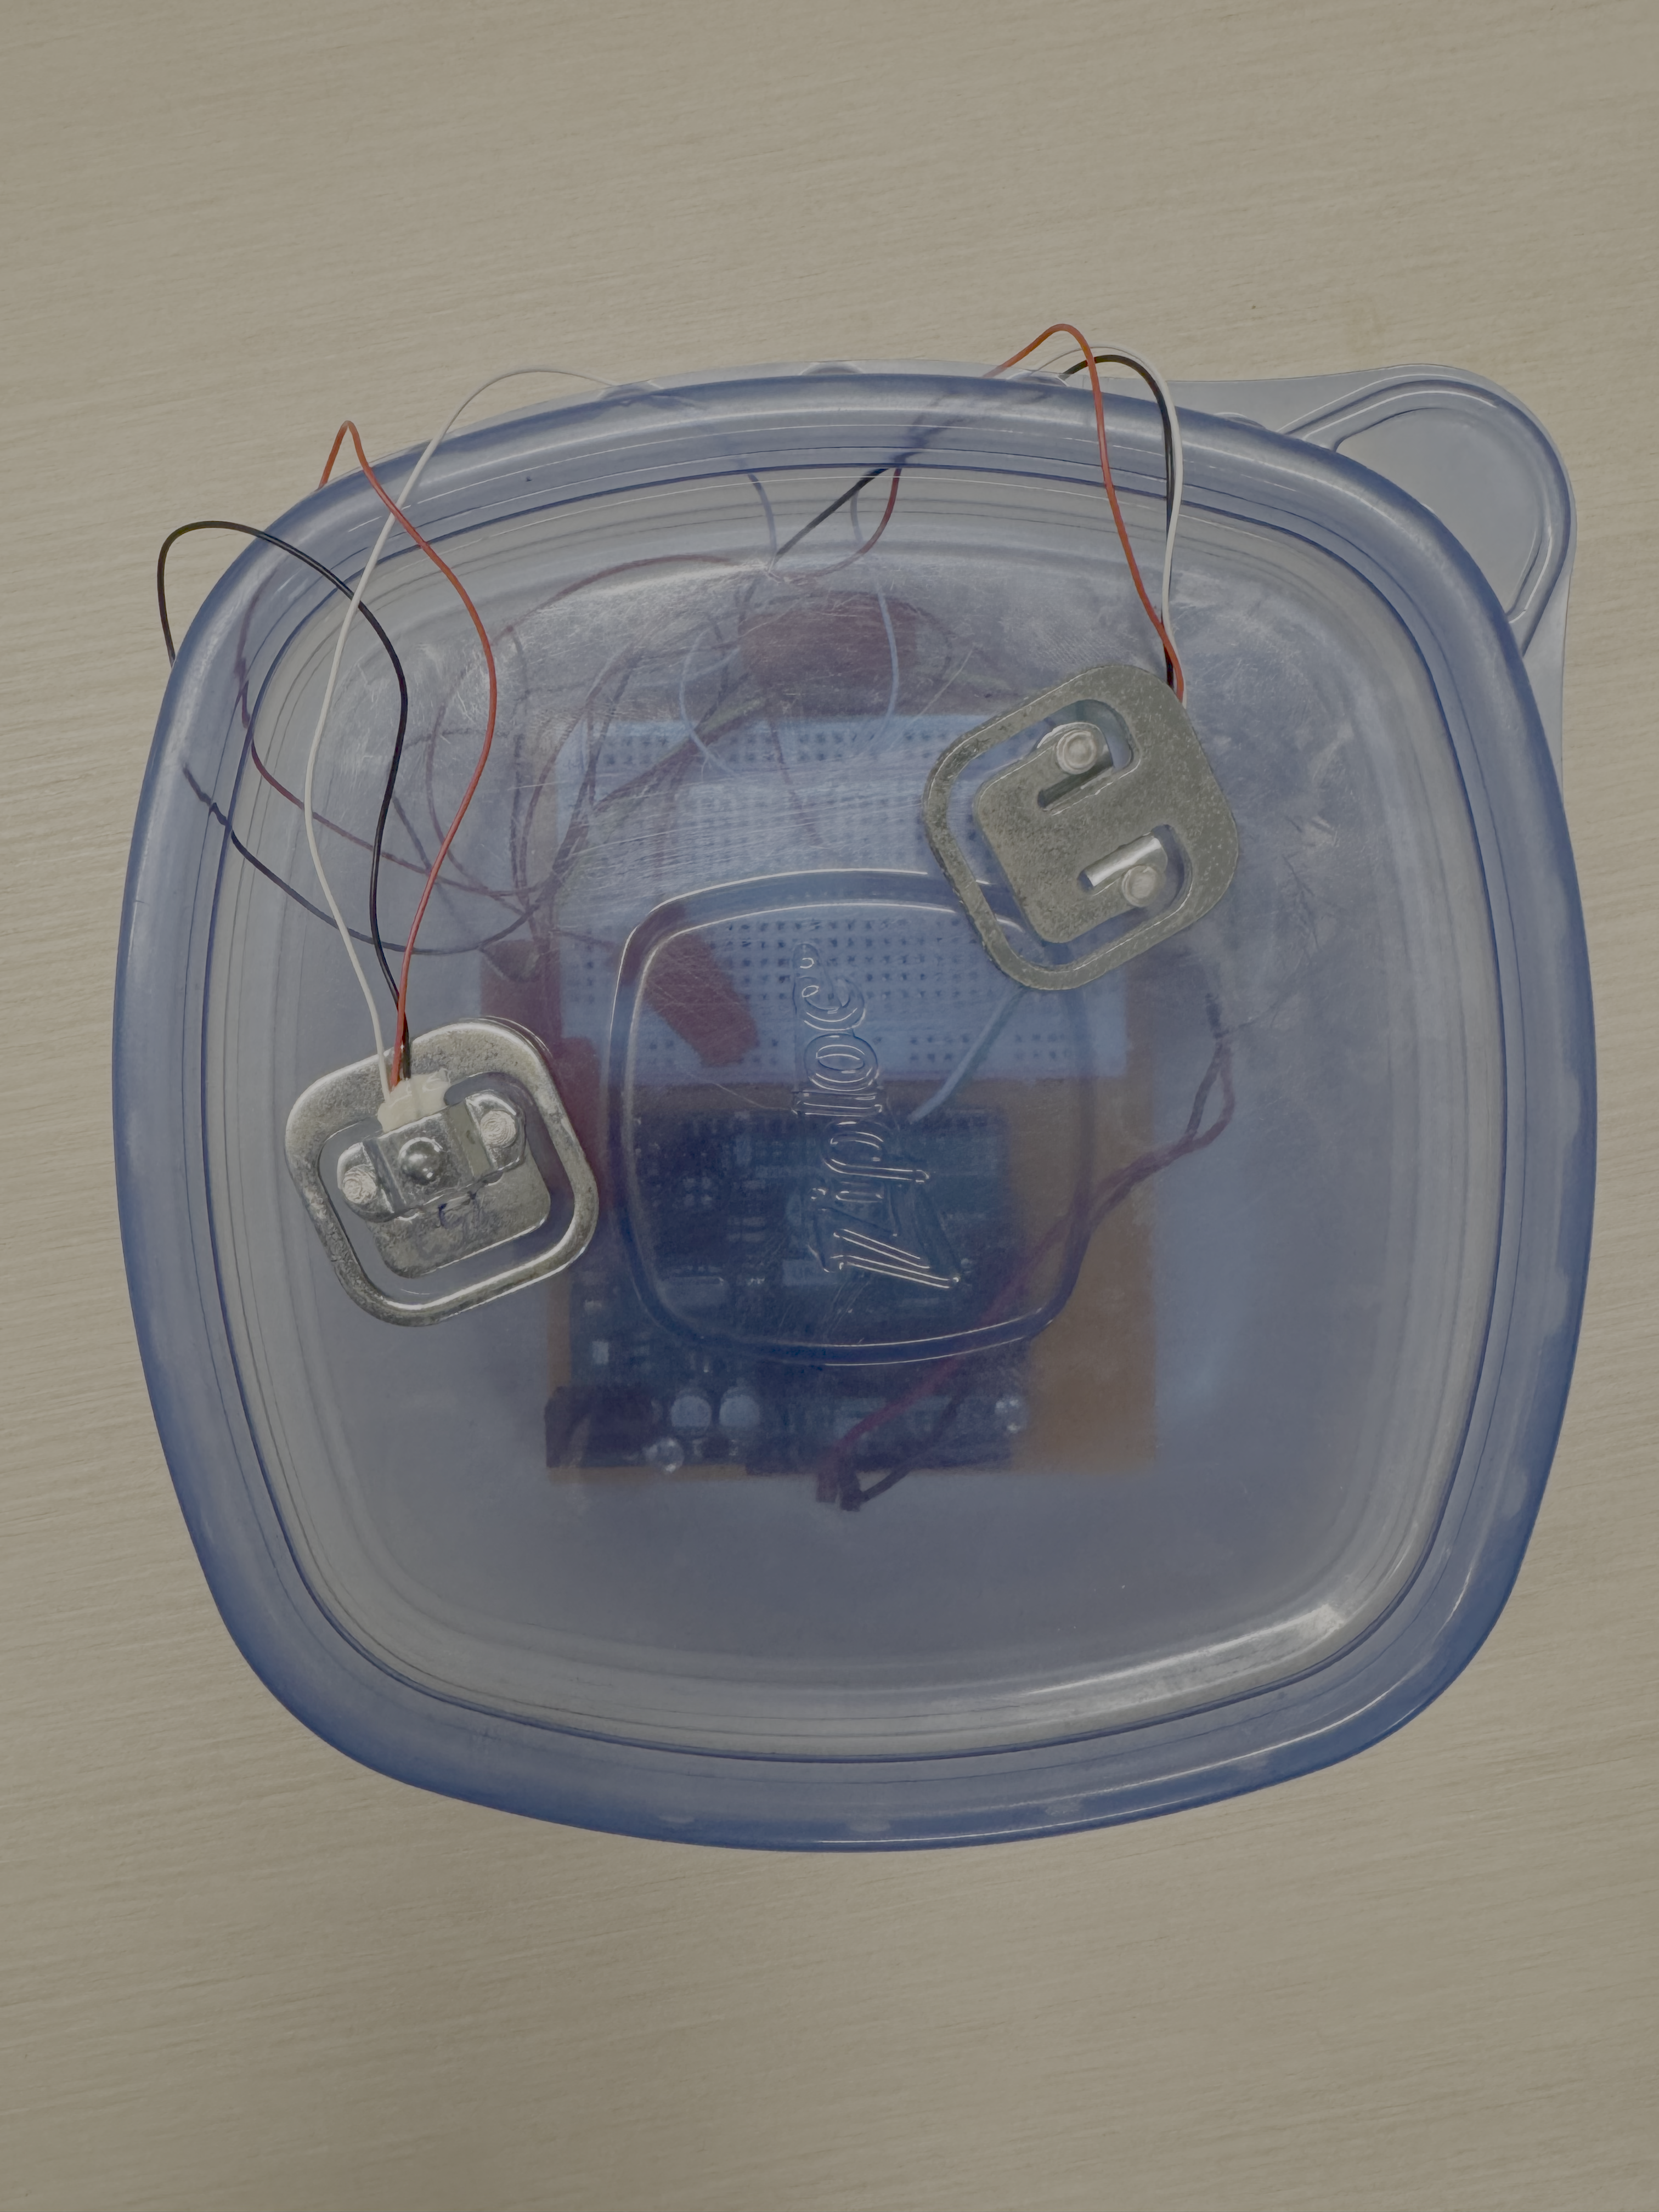
\includegraphics[width=0.9\linewidth]{closed.png}
  \caption{The electronics can be concealed, satisfying the concealement requirement.}
\end{subfigure}%
\begin{subfigure}{.5\linewidth}
  \centering
  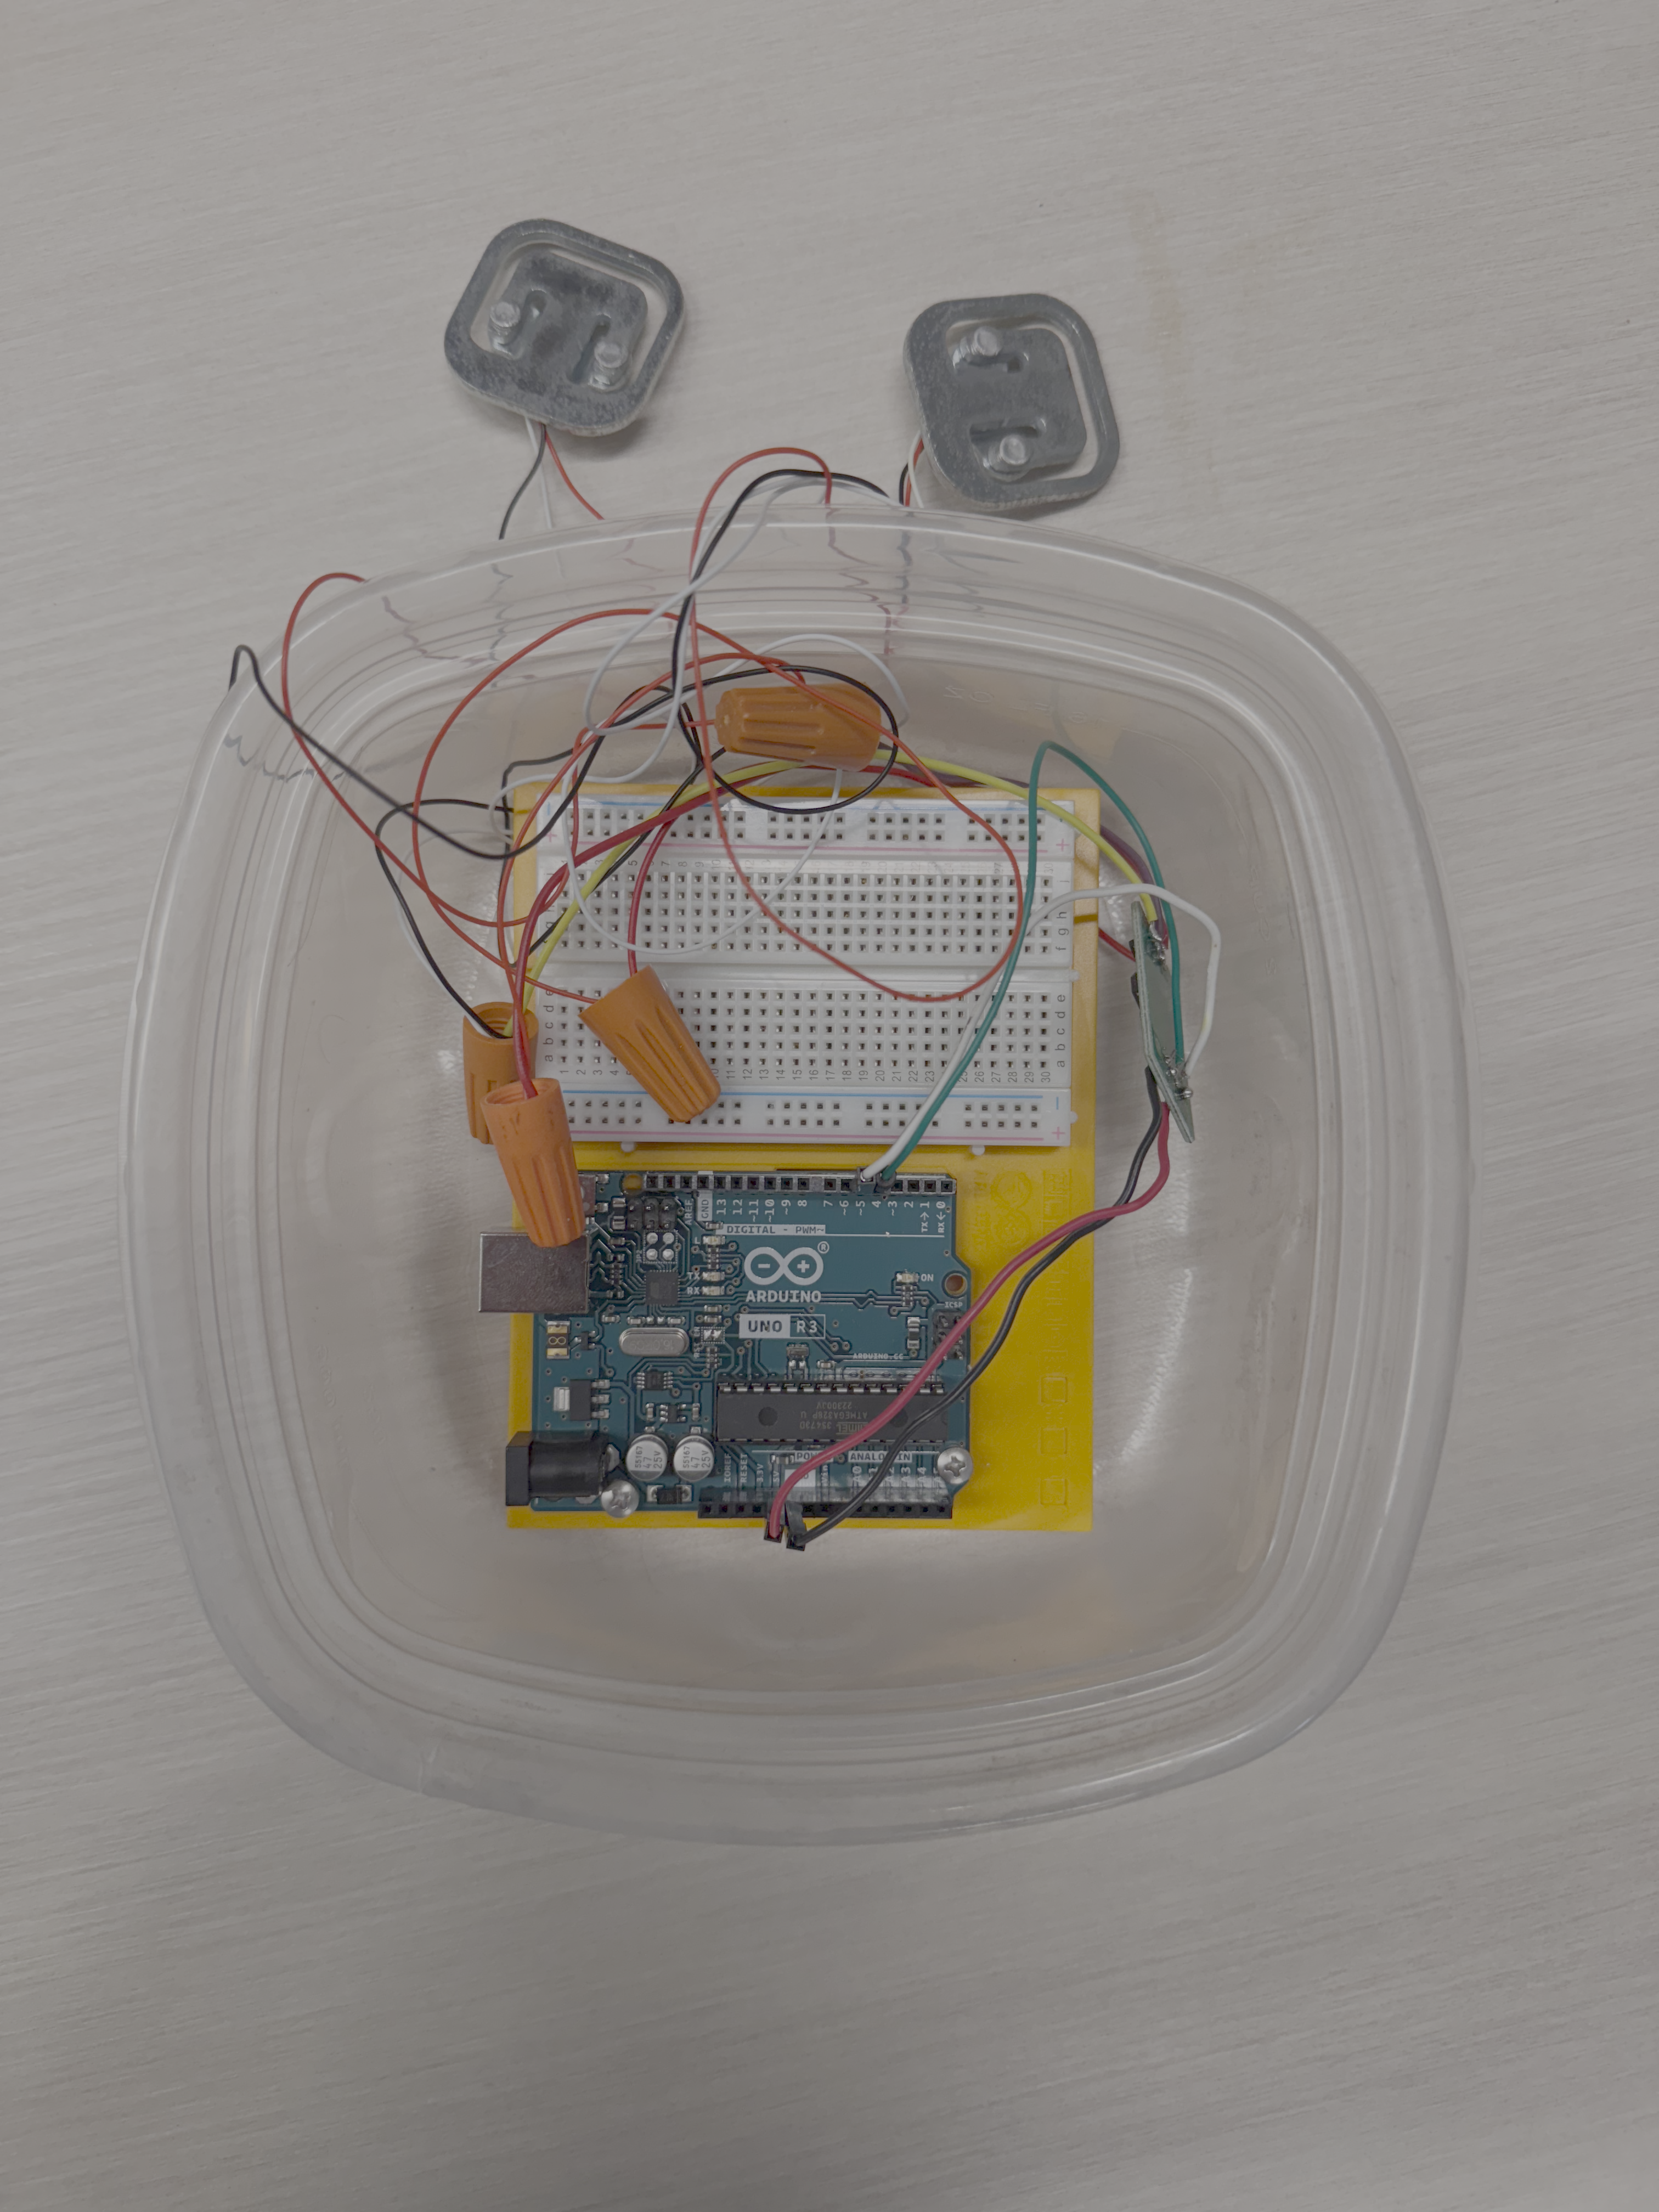
\includegraphics[width=0.9\linewidth]{inside.png}
  \caption{The internals of the pressure sensor prototype}
  \end{subfigure}
\caption{Minimally operational prototype of the pressure sensor design concept. The completed design connects the sensor to a notification device of the users choice.}
\label{fig:pressureSensorPhoto}
\end{figure}

We did not choose this design as it was also worse than others in the most important requirement: fixing back posture, for the same reason as the pokey belt. As well, the electronics in the design make it worse in the safety requirements, as mechanical designs of similar complexity are usually safer since they do not have voltage or frequency concerns.
\subsection{Changing The Seating Angle To Make Good Posture Comfortable: The Inclined Pillow}

Our final design for comparison is an inclined pillow. It is made of memory foam, which meets our safety requirements (requirements 2 and 10). The design is adjustable as it has a metal slider that changes the geometry of the pillow. This allows the user to modify the shape so that leaning backward and having good posture becomes the most comfortable position, which the user then adopts. The section that is in contact with the user is made out of memory foam and is designed to be wide enough to fit the 5th percentile EngSci female to the 95th percentile EngSci male, as per modified standard design practices. 

\begin{figure}[H]
\centering
\begin{subfigure}{.5\linewidth}
  \centering
  \includegraphics[width=0.9\linewidth]{pillow.jpg}
  \caption{Wooden prototype of the inclined pillow.}
\end{subfigure}%
\begin{subfigure}{.5\linewidth}
  \centering
  \includegraphics[width=1.0\linewidth]{CAD.jpg}
  \caption{CAD model of the inclined pillow. This stripped-down model shows the mechanical part that allows the user to adjust their seating angle.}
  \end{subfigure}
\caption{Basic operational prototype of the inclined pillow design concept. Memory foam and casing will be added to the actual design.}
\label{fig:pillow}
\end{figure}

We did not choose this design as it is more complicated than the shoulder straps, and our team values simplicity. The increased mechanical complexity can lead to less durability and ease of use. Furthermore, the use of this design requires a backed chair, limiting the design's use. Lastly, this design is less portable than the other options, as it is bulkier and heavier than other designs.


\section{Process Used To Create And Rank Designs} %ref other designs
\subsection{Diverging}
The diversity between the diverging tools we used, ``Brainwriting 4-3-3",  ``Lotus-Blossom", ``Bio-mimicry", and ``Random Input", enabled us to explore the entire scope of the design space before converging (Figure 6). These specific tools were chosen as they had varying approaches to diverging, allowing us to explore the design space from different perspectives.

\begin{figure}[H]
\centering
\begin{subfigure}{.5\linewidth}
  \centering
  \includegraphics[width=0.6\linewidth]{real random.png}
  \caption{Random words.}
\end{subfigure}%
\begin{subfigure}{.5\linewidth}
  \centering
  \includegraphics[width=0.6\linewidth]{real lotus.png}
  \caption{Lotus Blossom Technique}
  \end{subfigure}
\caption{Some of the diverging tools we used to come up with our designs.}
\label{fig:divergingTools}
\end{figure}

\subsection{Converging Onto And Comparing Prototypes}
With the prototypes that aligned with our requirements, the converging process used our evaluation criteria to determine which design would work best for our primary stakeholder. Each tool used during the converging process. explained below, had some limitations, which needed to be addressed to equitably explore the design space.
\subsubsection{A Pugh Chart With Some Bias}

\begin{figure}[H]
    \centering
            \includegraphics[scale=0.5]{image.png}
                \caption{This Pugh chart shows our evaluation process for determining the best prototype. There are more requirements on electronics, suggesting a simpler physical prototype is more efficient.}
            \label{fig:pughChart}
\end{figure}

The Pugh chart presents the shoulder straps as the most viable and fitting design. However, this model possesses limitations. Due to the diverse nature of our designs, the shoulder straps were evaluated the highest on most evaluation criteria as they emphasized simplicity. We purposefully included a slight bias in our requirements and evaluation criteria towards simpler, non-electronic citations since our group values ease of use and design simplicity.

However, there may be benefits to using technology that would be overlooked in our evaluation criteria framework, such as being able to track posture throughout the day and weeks, which would allow the user to see the trend line of improvement throughout an extended period of time. To acknowledge our biases and to avoid looking at a design space that is too narrow, we compared two different approaches of addressing the opportunity: The simpler shoulder straps and the more complex electronic pressure sensor. During the initial diverging phase, we thought our strongest prototype was the pressure sensor, due to its innovation, instant feedback and relative ease of manufacturing for an electronic device. Thus, we performed a pairwise comparison between the pressure sensor and shoulder straps, helping us to arrive to the best solution from two separate design spaces. 

\subsubsection{Using Pairwise Comparison To Determine That Shoulder Straps Are Better}

\begin{figure}[H]
\caption{Pairwise comparison table comparing the shoulder strap and pressure sensor designs. The most important criteria include simplicity and ease of use, which is why the shoulder strap design outperforms the more complex pressure sensor, at least according to what our team values.}

\begin{xltabular}{\linewidth}{X X}
Shoulder Straps & Pressure Sensor  \\ [1 ex] \hline
- No electromechanical parts & - Portable \\
- Constrictive and provides pressure feedback & - Provides instant feedback and notification based tracking throughout day \\
- Safer to use (no voltage) & - Positive reinforcement to train back muscles \\
- No protrusion since it's worn & - Less pressure on shoulder \\
- Durable & -  Less volume 
\end{xltabular}

\label{comparisontable}
\end{figure}

From psychological research studying the best method to maintain healthy posture\cite{RefWorks:70} and the results of the pairwise comparison, the shoulder straps outperform the pressure sensor in actively correcting long-term back posture. They are worn, are more portable and have fewer mechanical parts, satisfying our biggest requirements. Consequently, the shoulder straps are chosen as the recommended design concept. 

\section{Final Recommendation Of Shoulder Straps To Fix Back Posture}
We recommend the shoulder strap design because it is a viable and proven prototype that could gradually correct back posture amongst EngSci students when sitting on chairs with backs. This prototype includes quick-release straps, folds to fit inside a small lunch bag, has a polyester string to ensure breathability and flexibility, and incorporates traditional memory foam for comfort and low pressure. The design was inspired by suspenders and back braces, which did not adhere to the specific requirements frameworks of our stakeholders. Consequently, our goals targeted portability, safety, aesthetics, durability, and  the ability to correct back posture, so they are more suitable to our stakeholders. 
Upon exploring the design space, we assessed our four different designs that best aligned with our requirements. The shoulder straps best fits the posed evaluation criteria. They performed better than most designs in our most important criteria, and avoid using materials that might pose a safety hazard altogether. Additionally, it is designed for manufacturability and simplicity, providing more benefits to stakeholders. Given that there was no preference for technological devices, it was deemed that shoulder straps were better since they do not have electromechanical components and voltage. This aligned with our teams values, and we believe it is the best option out of the proposed solutions to fix EngScis poor posture.


\includepdf[pages=-, scale=1.0, pagecommand={\thispagestyle{plain}}]{refv3.pdf}
\begin{appendices}
\section{Stakeholder Interview Results}
Responses from interviews conducted to a sample of 11 students show that even though they are conscious of their poor posture, they do not want to use any of the current designs due to the following factors: 
\begin{enumerate}
\item Societal expectations: Students do not want to feel like outcasts in society or be seen as “nerds” 
\item One of the current designs (lumbar pillow) continuously slips and is uncomfortable 
\item Students found it annoying to have to put it on every time 
\item Current designs can be annoying to carry around 
\item Another design (back braces) is too obvious and visible 
\end{enumerate}
\label{appendix:inteviews}
\section{Design Brief}
\includepdf[pages=1-9, scale=0.9, pagecommand={\thispagestyle{plain}}]{Design Brief Draft.pdf}
\label{appendix:designBrief}
\section{Video Link}
\href{https://youtu.be/jkqF1FlfK5o}{Testing Requirements - Praxis Design Report: https://youtu.be/jkqF1FlfK5o}
\end{appendices}

\end{document}